\chapter{Empirisk studie av regelbasert orddeler}

I dette kapittelet ser vi på testingen av Hyphenator-programmet. Først spør vi hvilke spørsmål vi ønsker svar på, og definerer problemstillingene for oppgaven. Deretter blir metodene og målene for testene diskutert. Til slutt i dette kapittelet presenteres resultatene, før vi avslutter med en diskusjon rundt funnene og knytter dem opp til problemstillingene. 

\section{Problemstilling}

Det er mange aspekter som kunne vært testet, men det er spesielt to spørsmål som er interessante å få svar på i denne sammenhengen.

\begin{quote}
PS1: Hvor godt utfører modulene oppgavene sine hver for seg?
\end{quote}

Det vil være interessant å se nærmere på modulene i isolasjon med egne testkriterier og tester. Med dette vil det være mulig å identifisere svakheter i enkeltmoduler i programflyten, og kan fungere som en pekepinn på mulig videre arbeid for å forbedre programmet.

\begin{quote}
PS2: Hvor god kvalitet og kontroll får vi på orddelingen?
\end{quote}

Her ønsker vi å få svar på hvor vellykket løsningen er for å dele ord, samt eventuell hvilken økt kontroll vi kan få over orddelingsvalgene.

\section{Metode}

I forbindelse med \term{PS1} er det følgende moduler som er av interesse å teste: CompoundSplitter: \textit{hvor godt finner den alle mulige dekomponeringer av et sammensatt ord?} CoumpoundInterpreter: \textit{i hvor stor grad velger den riktig tolkning ved flere muligheter?} Og HyphenationRules: \textit{hvor godt påfører den reglene på ikke-sammensatte ord?} Dictionary og EphenthesisAnalyser vil ikke bli testet, da førstnevnte kun vil fungere som en hjelpemodul, og sistnevnte testes indirekte gjennom CompoundInterpreter. Ved \term{PS2} vil helheten av programmet og samspillet mellom modulene testes.

\subsection{PS1}

Her ser vi på metodikken benyttet for å belyse spørsmålet som er formulert i \term{PS1}, hvor vi ønsker å se nærmere på modulene individuelt.

\subsubsection{CompoundSplitter}

Denne modulen har som oppgave å dekomponere sammensatte ord til alle lovlige dekomponeringer, hvor ønsket dekomponering er en del av resultatmengden. Modulen vil utsettes for to tester. En \term{triviell test}, som består av 152 enkelt sammensatte ord. Det vil si ordsammensetninger som typisk har nullfuge og består av to rotord. Dette for å teste hvor godt modulen fungerer i de enkleste tilfellene, som også er formen til majoriteten (75 \%) av alle sammensatte ord i norsk \cite{johannessen1996automatic}. Den andre testen vil være en \term{kompleks test}, bestående av 27 sammensettninger som kan ha flere rotordkomponenter, samt kan inneholde binde-s eller binde-e. Slik får vi testet mer komplekse, sammensatte ord, som kan være mer vanskelig å dekomponere korrekt. De fleste av sammensetningene er hentet fra Hauglin og Johannesen \cite{johannessen1996automatic}, som er konstruerte eksempel for å illustrere spesielt vanskelige ordsammensetninger med og uten bindebokstav.

Vi registrerer et resultat som korrekt når ønsket dekomponering er en del av resultatmengden som returneres fra modulen.

\ex{eplekake}{(inndata, ønsker eple+kake)}\newline
\exx{[[ep, le, kake], [eple, kake]] (gyldig løsn.)}{}

\paragraph{Mål} I denne komponenten ønsker jeg å finne \textit{alle} lovlige dekomponeringer, og at ønsket dekomponering er en del av løsningsmengden. Denne testen bør resultere i opp mot 100 \% korrekte resultater. 
	
\subsubsection{CoumpoundInterpreter}

For denne modulen ønsker jeg å gjøre to tester: én med enkle sammensatte ord med nullfuge fra Norsk ordbank, da denne formen for komposisjon er det desidert mest frekvente (75 \% av alle sammensatte ord har nullfuge\cite{johannessen1996automatic}). I test nummer to kommer jeg til å bruke en liste over ekstra problematiske sammensatte ord som er to- eller flertydige, og som eventuelt inneholder binde-s eller binde-e. Flere av disse eksemplene vil jeg hente fra Johannesen og Hauglin \cite{johannessen1996automatic}, da flere av disse er konstruert for å illustrere vanskelighetene ved sammensatte ord med bindebokstaver. Slik vil også modulen EphenthesisAnalyser bli testet indirekte.

Hva som er en korrekt tolkning av et sammensatt ord er ikke helt enkelt å gi et entydig svar på. Men et kriterium er at det bør være mest mulig likt slik et menneske intuitivt ville tolket det. \textit{Lesesals+turer} fremfor \textit{lesesal+sturer} og \textit{dop+lager} fremfor \textit{do+plager} (tolkning som er litt mer i gråsonen). Mange av disse tolkningene vil være kontekstavhengig, som kan gjøre det vanskeligere for leseren å tolke.

\paragraph{Mål} Siden jeg støtter meg på metodene til Sjöberg og Kann \cite{sjobergh2004finding} bør det forventes å kunne få like god tall som hans enkleste, men også effektive, metode som kun ser på \textit{antall komponenter i tolkningen} (prøver å redusere). Resultatene hans ga 90 \% korrekte tolkninger ved analyse av sammensatte ord med flere mulige tolkninger (flertydige). Vi introduserer også en noe mer avansert tolkning av bindebokstaver enn det Sjöberg og Kann gjør, så det bør forventes bedre resultat enn 90 \% i begge tester.

\subsubsection{HyphenationRules}

For å isolere ut denne modulen og teste nøyaktigheten til den alene, vil jeg konstruere en liste med ikke-sammensatte ord, som jeg også deler manuelt etter reglene for orddeling. Ordlisten for ikke-delte ord vil bli matet inn i modulen, og forsøkt delt. Så gjøres det en sammenligning mellom resultat og den hånddelte listen av ord. Der vil jeg se på prosentandelen av G (good), antall riktige delepunkter funnet, B (bad), antall falske negativer og M (missed), antall falske positiver.

\paragraph{Mål} Denne testen gjøres kun med ikke-sammensatte ord, og vil derfor være enklere å utføre siden mye av kompleksiteten ved å påføre orddelingsreglene er nettopp ved analysen av sammensatte ord. Thoresen \cite{thoresen1993virtuelle} sine resultater er en naturlig sammenligning, og det bør forventes noe bedre resultater en hva han presenterer, 90,5 \% korrekte og 0,97 \% falske positiver.

\subsection{PS2}

Helheten vil bli testet med en større liste over (sammensatte og ikke-sammensatte) ord. For å kunne sjekke om disse deles korrekt, er vi avhengig av å ha en kontrolliste over korrekte delinger vi kan sammenligne med. Som beskrevet i kapittel~\ref{sec:ordlister} er det vanskelig å få tak i lister over norske ord med alle korrekte delepunkter. Jeg vil derfor støtte meg til listen konstruert av Lars Gunnar Thoresen \cite{thoresen1993virtuelle}. Listen\footnote{Listen over delte ord er tilgjengelig som vedlegg i Lars Gunnar Thoresen sin masteroppgave på \url{https://www.duo.uio.no/handle/10852/8875}.} er konstruert av $16226$ ord valgt ut fra et representativt tekstkorpus fra skjønnlitteratur og blandet faglitteratur, allmennfaglig nyhetsstoff og faglitteratur informatikk. De mest hyppige ordene ble valgt ut gjennom en frekvensanalyse. Ved å bruke samme testdata som Thoresen, vil det også være mulig å sammenligne mine resultater med det han fikk gjennom patgen og \TeX{}-algoritmen. Som med HyphenationRules, vil jeg her se på å prosentandelen av G (good), antall riktige delepunkter funnet, B (bad), antall falske negativer og M (missed), falske positiver.

\paragraph{Mål} Igjen er det naturlig å sammenligne med resultatene til Thoresen. For at tilnærmingen jeg presenterer skal være av interesse for bruk, bør den løse oppgaven med å dele ord minst like godt. 

\section{Resultater}

Jeg ønsket først å teste alle modulene hver for seg, før jeg så testet hele systemet samlet. Dette for i større grad kunne identifisere hvor eventuelle feil oppsto og i hvilke komponenter, for så å kunne klassifisere feilene bedre. Fremgangsmåten og ønskede resultater ble beskrevet i forrige kapittel. I denne teksten vil jeg beskrive hvordan testene faktisk ble gjennomført, for så å vise resultatene og tolke resultatene.

\subsection{PS1}

Her vil jeg videre presentere resultatene knyttet til PS1 i forbindelse med modulene.

\begin{table}[h]
	\centering 
	\begin{tabular}{llrrrr} \hline 
		\textbf{Navn} & \textbf{Type} & \textbf{Korrekt} & \textbf{Feil} & \textbf{(Av)} & \textbf{\%} \\
		\hline \multirow{2}{*}{\textbf{CompoundSplitter}} & Enkel & 150 & 2 & 152 & 98,68 \\
		\cline{2-6} & Kompleks & 27 & 0 & 27 & 100 \\
		\hline \multirow{2}{*}{\textbf{CompoundInterpreter}} & Enkel & 89 & 6 & 95 & 93,68 \\
		\cline{2-6} & Kompleks & 70 & 12 & 82 & 85,36 \\
		\hline 
	\end{tabular}
	\caption[Oppstilling av testresultater av moduler]{Oppstilling av resultatene fra testing av CompoundSPlitter og CompoundInterpreter, knyttet til PS1.} \label{tab:module-test} 
\end{table}

\subsubsection{CompoundSplitter}

Av tabell~\ref{tab:module-test} ser vi at modulen fikk alle riktige for den komplekse testen, og 98,68 \% riktig på den enklere testen. De to feilene som oppsto i den enkle testen er følgende (diskutert i kapittel \ref{sec:disk-ps1}):

\ex{acappella+sang}{(feil: acapellasang)}\newline
\exx{av+hør}{(feil: av+hør)}

\subsubsection{CompoundInterpreter}

Testen av CompoundInterpreter med enkelt og kompleks test, ga korrekt resultat i  henholdsvis 93,68 \% og 85,36 \% av tilfellene. Resultatet diskuteres videre i kapittel~\ref{sec:disk-ps1}, hvor også eksempler av feiltolkninger listes opp.

\subsubsection{HyphenationRules}

HyphenationRules-modulen ble testet med én liste med ikke-sammensatte ord. Resultatet vises i tabell~\ref{tab:hyphenation-results}. Prosentvis gir det G, B, M på henholdsvis 98,03 \%, 0,98 \% og 1,96 \%. Tre feil oppsto. «ar-be-id» ble delt som «Ar-beid», grunnet manglende implementasjon av støtte for deling mellom vokaler som hører til hver sin stavelse. «Ang-re» blir delt «an-g-re», som skyldes at det blir feiltolket «an» som et avledningsprefiks. «Vis-s-te» som blir det «viss-te». Her er jeg noe mer usikker på hvorfor «vis-s-te» deles slik det gjør i fasiten. Det kan være en feiloppføring, eller at «ste» regnes som bøyningsendelsen til ordet «vite».

\subsection{PS2}

I forbindelse med PS2 ble tre aspekter testes. Først en enkel test med ikke-sammensatte ord som tester modulen for påføring av orddelingsreglene direkte – uten å gå gjennom modulene for dekomponering. Deretter ble hele programmet testet med orddelingslisten på 16.226 ord, fra Thoresen \cite{thoresen1993virtuelle}. Resultatene kan sees i tabell~\ref{tab:hyphenation-results}. I forbindelse med den komplette testen, ble også eksekveringstid registrert. Det ga 45 sekunder for innlasting av ordliste i trie-struktur, og 36 sekunder for deling og resultatsammenligning av alle $16226$ ord. 

\begin{table}[h]
	\centering 
	\begin{tabular}{llrrrr} \hline 
		\textbf{Navn} & \textbf{Type} & \textbf{G} & \textbf{B} & \textbf{M} & \textbf{(Av)} \\
		\hline \textbf{HyphenationRules} & Enkel & 100 & 1 & 2 & 102 \\
		\hline \textbf{Hyphenator} & Komplett & 31439 & 3694 & 7507 & 38946 \\
		\hline 
	\end{tabular}
	\caption[Resultater fra test av Hyphenator-programmet]{Oppstilling av resultatene fra enkel og komplett test av orddelingsalgoritmen. Enkel test er utført med kun ikke-sammensatte ord, komplett test består av 16.226 ord hentet fra Thoresen \cite{thoresen1993virtuelle}. G (Good) beskriver antall korrekte delepunkter funnet, B (Bad) beskriver falske negativer og M (Missed) beskriver falske positiver.} \label{tab:hyphenation-results} 
\end{table}

Siste aspekt som skulle testes var i forbindelse med kontroll over delepunkter og orddelingsregler benyttet. Her skulle egentlig alle orddelingsreglene testes individuelt. Av tidshensyn har kun ordleddsregelen om deling i sammensetningsfugen av sammensatte ord blitt testet. Dog kan det poengteres at dette er en av de viktigste reglene, som gir de peneste delingene med minst rom for forvirrende ordbilder (slik de andre reglene, spesielt enkonsonantregelen kan skape). Resultatet fra testen er stilt opp i tabell~\ref{tab:ordleddsregelen}.

\begin{table}[h]
	\centering 
	\begin{tabular}{lrrrr} \hline 
		\textbf{Navn} & \textbf{G} & \textbf{B} & \textbf{M} & \textbf{(Av)} \\
		\hline \textbf{Ordleddsregelen} & 24 & 9 & 6 & 30 \\
		\hline 
	\end{tabular}
	\caption[Resultater fra test av ordleddsregelen]{Oppstilling av resultatet fra test av ordleddsregelen. Tegnforklaringen er den samme som beskrevet i tabell~\ref{tab:hyphenation-results}} \label{tab:ordleddsregelen} 
\end{table}

\section{Diskusjon}

I resten av kapittelet vil vi vende tilbake til de to problemstillingene, og diskutere dem knyttet opp til resultatene presentert tidligere. Til slutt tar vi et kritisk blikk på eget arbeid.

\subsection{PS1: Hvor godt utfører modulene oppgavene sine hver for seg?}
\label{sec:disk-ps1}

Av tabell \ref{tab:module-test} kan vi se at modulen CompoundSplitter fungerer svært godt. Den komplekse testen får korrekt resultat for alle sammensatte ord, mens den enkle testen får 98,68 \% korrekte resultater, med kun to feil. Disse feilene er mulig å rette opp. Første feil er ordet «avhør», som ikke returnerer som «av+hør». Dette skyldes at «av» blant annet er listet i ordboken som en forkortelse (for audio-visuelt), og dermed vil Dictionary-modulen si at oppslaget av ordet ikke er et gyldig ord. Dette kan enkelt løses ved at modulen svarer at det er et gyldig ord, så lenge det finnes minst én oppføring som ikke er en forkortelse. Den andre feilen er «acappellasang», som kun returnerer det samme ordet og ikke «acappella+sang». Dette skjer fordi ordlisten ikke har «acappella» som en oppføring for seg selv. I slike tilfeller hvor eventuelt deler av et sammensatt ord ikke er kjent for ordboken, foreslår Johannesen og Hauglin at man søker etter det lengste prefikset eller suffikset av strengen som er kjent for ordboken, og deler ordet i denne fugen. Eksempelvis ordet «ibsenstykket», hvor «stykket» er lengste suffiks, vil deles som «ibsen+stykket». Med begge testene oppnådde vi målet om tilnærmet 100 \% korrekte resultater.

Modulen CompoundInterpreter fungerer ikke tilstrekkelig godt nok. For den enkle testen ønsket vi å oppnå minst 97 \% korrekte tolkninger, og 94 \% for den komplekse testen. Med resultater på henholdsvis 93,68 \% og 85,36 \% ser vi at avstanden er for stor. Når Johannesen og Hauglin i tillegg hevder å få feil tolkning av sammensatte ord i kun 1,1 \% av tilfellene, ser vi her at det gjenstår en del videre arbeid for at denne modulen oppfyller kravet om å være tilstrekkelig god. Ved å studere feilresultatene fra begge testene, er det tydelig to kategorier av feil som opptrer desidert hyppigst og fører til dårlige resultater. Den første er ikke-sammensatte ord som blir tolket som sammensatte.

\ex{etter → et+ter}{}\newline
\exx{også → og+så}\newline
\exx{sier → si+er}{} 

Dette skyldes vanskeligheten med å avgjøre om et ord er sammensatt eller ikke. Dette diskuteres ytterligere i kapittelet for videre arbeid, \ref{sec:videre-arbeid}. Den andre kategorien for feil, er tolkninger hvor vi får en for høy prioritering på  valg tolkninger med det lengste etterleddet (beskrevet i kapittel \ref{sec:comp-int}). 

\ex{brakkvann → brak+kvann}{}\newline
\exx{førtitall → før+titall}{}\newline
\exx{flislegger → fli+slegger}{}\newline
\exx{hustak → hu+stak}{}\newline
\exx{blomsterholder → blomst+erholder}{}

\subsection{PS2: Hvor god kvalitet og kontroll får vi for orddelingen?}

\marginelement{
\begin{tikzpicture}
  \centering
  \begin{axis}[
        ybar, axis on top,
        %title={Sammenligning av resultater},
        ymajorgrids, tick align=inside,
        major grid style={draw=white},
        enlarge y limits={value=.1,upper},
        width = \marginparwidth,
		height = 7cm,
        ymin=0, ymax=100,
        axis x line*=bottom,
        bar width = 0.08\textwidth,
        axis y line*=right,
        y axis line style={opacity=0},
        tickwidth=0pt,
        enlarge x limits=true,
        yticklabel={\pgfmathparse{(int(\tick))}\pgfmathresult \%},
        legend style={
            at={(0.5,-0.01)},
            anchor=north,
            legend columns=-1,
            /tikz/every even column/.append style={column sep=0.5cm}
        },
        %ylabel={Prosent (\%)},
        symbolic x coords={
           Good,
           Bad,
          Missed},
       xtick=data,
       nodes near coords={
        \pgfmathprintnumber[precision=2]{\pgfplotspointmeta}
       }
    ]
    \addplot [draw=none, fill=red] coordinates {
      (Good,98.03)
      (Bad,0.98)
      (Missed,1.96) };\label{meg}

    %\legend{Meg,Gunnar}
  \end{axis}
  \end{tikzpicture}
    \captionof{figure}{Oppstilling av resultater fra den enkle testen av orddelingsalgoritmen gjort på en liste over ikke-sammensatte ord.}
    \label{fig:simple-result}
}

Målet for kvalitet, det vil si antall positiver (G), antall falske negativer (B) og antall falske positiver (M), var satt til å være minst like gode som Lars Gunnar Thoresen sine resultater for sine norske orddelingsmønstere for \TeX{}-algoritmen. Resultatene fra den enkle teste, bestående av ikke-sammensatte ord, ga gode resultater (se figur~\ref{fig:simple-result}). Prosentvis mengde falske negativer (B) er så og si identisk med Thorsen sine resultater (0,97~\%). Samtidig finner vi en stor andel flere positiver (G). 

I figur~\ref{fig:results} kan vi se en sammenstilling av resultatene fra den komplette testen av samme ordliste, bestående av $16226$ ord, som Thoresen benyttet seg av. Her ser vi konsekvent at resultatene for Hyphenator slår dårligere ut enn sammenligningen. Spesielt er antall falske negativer uakseptabelt høy. For en orddelingsalgoritme er det viktigere med lavest mulig antall feil delepunkter, enn det er å finne alle mulige delepunkter. Når ord skal deles ved linjeskift, trenger vi stort sett bare ett korrekt delepunkt. Mens et feil delepunkt kan fort føre til et misvisende eller komisk ordbilde.

\begin{figure}[h]
	\begin{tikzpicture}
  \centering
  \begin{axis}[
        ybar, axis on top,
        %title={Sammenligning av resultater},
        ymajorgrids, tick align=inside,
        major grid style={draw=white},
        enlarge y limits={value=.1,upper},
        width = \textwidth,
        height = 6cm,
        ymin=0, ymax=100,
        axis x line*=bottom,
        bar width = 0.08\textwidth,
        axis y line*=right,
        y axis line style={opacity=0},
        tickwidth=0pt,
        enlarge x limits=true,
        yticklabel={\pgfmathparse{(int(\tick))}\pgfmathresult \%},
        legend style={
            at={(0.5,-0.01)},
            anchor=north,
            legend columns=-1,
            /tikz/every even column/.append style={column sep=0.5cm}
        },
        %ylabel={Prosent (\%)},
        symbolic x coords={
           Good,
           Bad,
          Missed},
       xtick=data,
       nodes near coords={
        \pgfmathprintnumber[precision=2]{\pgfplotspointmeta}
       }
    ]
    \addplot [draw=none, fill=red] coordinates {
      (Good,80.72459302624146)
      (Bad,9.48492784881631)
      (Missed,19.27540697375854) };\label{meg}
   \addplot [draw=none,fill=bar] coordinates {
      (Good,90.50) 
      (Bad,0.97)
      (Missed,9.50) };\label{gunnar}

    %\legend{Meg,Gunnar}
  \end{axis}
  \end{tikzpicture}
  \caption[Sammenstilling av resultater fra \TeX{} og Hyphenator]{Sammenstilling av resultater fra Hyphenator (\ref{meg}) og \TeX{}-algoritmen (\ref{gunnar}) med mønstere fra Lars Gunnar Thoresen. Good, antall positiver funnet, ønsker vi høyest mulig, mens Bad, antall falske negativer og Missed, antall falske positiver, ønsker vi lavest mulig.}
  \label{fig:results}
\end{figure}

Når det gjelder aspektet om kontroll og hvilke regler som benyttes over delepunkter og type delepunkter ønsket, var intensjonen å sette opp individuelle tester for alle reglene. Slik kunne vi fått et bedre bilde over grad av kontroll over delepunktene som ønskes. Av tidshensyn har vi gått bort fra dette, og kun utført en test av ordleddsregelen. Dog kan det argumenteres for at dette er den viktigste av reglene, som gir de «vakreste» delepunktene. Hvis deling etter ordleddsregelen utføres riktig vil muligheter for misvisende eller komiske ordbilder, slik vi kan se i figur~\ref{fig:dopalger} og \ref{fig:freskukens}, reduseres. Resultatet fra tetsten av ordleddsregelen er fremstilt i figur~\ref{fig:ordleddsregelen}. Resultatene, spesielt antall falske negativer (Bad) er ikke tilfredstillende. Men testen er svært liten og det er derfor vanskelig å konkludere entydige. Større og fler tester av reglene individuelt trengs.

\marginelement[-6]{

\includegraphics[width=\marginparwidth]{content/figures/forord-doplager.jpg}
\captionof{figure}[Eksempel på uheldig orddeling i Dagbladet]{Faksimile, Dagbladet Nett 25. september 2013. Eksempel på uheldig orddeling som fører til et komisk ordbilde. Trolig en feil ved ordleddsregelen og en feiltolkning at ordet er satt sammen av «do» og «plager». Kilde: \url{http://www.dagbladet.no/2013/09/25/nyheter/utdanning/narkotika/innenriks/29445603/}}
\label{fig:dopalger}
}

\marginelement[14]{
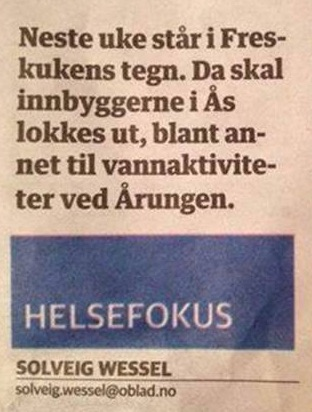
\includegraphics[width=\marginparwidth]{content/figures/freskukens.jpg}
\captionof{figure}[Eksempel på uheldig orddeling i Østlandet Blad]{Faksimile Østlandets Blad. Nok et eksempel på en uheldig orddeling. Muligens siden «fresk» eller «freskukens» var et ukjent ord for orddelingsprogrammet, og ordet ble delt etter enkonsonantregelen. Dette er en lovlig, men svært uheldig orddeling.}
\label{fig:freskukens}
}

\begin{figure}[h]
\centering
\begin{tikzpicture}
  \centering
  \begin{axis}[
        ybar, axis on top,
        %title={Sammenligning av resultater},
        ymajorgrids, tick align=inside,
        major grid style={draw=white},
        enlarge y limits={value=.1,upper},
        width = \marginparwidth,
		height = 7cm,
        ymin=0, ymax=100,
        axis x line*=bottom,
        bar width = 0.08\textwidth,
        axis y line*=right,
        y axis line style={opacity=0},
        tickwidth=0pt,
        enlarge x limits=true,
        yticklabel={\pgfmathparse{(int(\tick))}\pgfmathresult \%},
        legend style={
            at={(0.5,-0.01)},
            anchor=north,
            legend columns=-1,
            /tikz/every even column/.append style={column sep=0.5cm}
        },
        %ylabel={Prosent (\%)},
        symbolic x coords={
           Good,
           Bad,
          Missed},
       xtick=data,
       nodes near coords={
        \pgfmathprintnumber[precision=2]{\pgfplotspointmeta}
       }
    ]
    \addplot [draw=none, fill=red] coordinates {
      (Good,80.03)
      (Bad,30.0)
      (Missed,19.97) };\label{meg}

    %\legend{Meg,Gunnar}
  \end{axis}
  \end{tikzpicture}
    \caption[Resultater fra test av ordleddsregelen]{Oppstilling av resultater fra test av ordleddsregelen.}
    \label{fig:ordleddsregelen}
\end{figure}

\section{Svakheter}

Enkelte svakheter ved metodene benyttet under testingen er verdt å påpeke. Det første er at testene benyttet for å teste modulene individuelt er svært små. Det skyldes tidshensyn og det faktum at disse testene er i hovedsak ment for å vise eventuelle feil med modulene under utviklingsfasen. 

Den andre svakheten er ved den store orddelingsordlisten hentet fra Thoresen. Etter en gjennomgang av de tusen første ordene oppdaget jeg enkelte ord som var delt feil, som jeg fikk rettet opp. Men det kan antas at det vil finnes tilsvarende feildelte ord i resten av listen. Et annet problem avdekket ved listen er ordene som skal ha trippelskrevet konsonant ved orddeling, ikke er oppført riktig i listen. Alle ordene er konsekvent oppført som soppo-se, tallin-je, ka-jakklubb og fjelland, når du skulle vært sopp-po-se, tall-lin-je, ka-jakk-klubb og fjell-land. Disse er nok oppført slik bevisst, siden det er et kjent problem at orddelingsalgoritmen i \TeX{} ikke støtter slik ekspandering til trippelskrevne konsonanter. Dette problemet og andre problemer med \TeX{}-algoritmen, spesielt for språk som har ikke-standard orddeling, er påpekt i flere artikler \cite{sojka1995hyphenation,sojka1995notes,nemeth2006automatic,omega}.

Den tredje svakheten ligger i hvilken mønsterliste for \TeX{}-algoritmen som er valgt til sammenligning. Det er utviklet en nyere mønsterliste for norsk orddeling som nå distribueres med \TeX{}-systemet. En vil anta at disse mønstrene gir enda bedre resultater en mønstrene til Thoresen som sammenligningen gjøres mot. Men etter flere forsøk på henvedelser til forfatterene bak denne mønsterlisten lykkes det ikke å få tak i testresultatene for G, B og M-verdiene. Det ble derfor naturlig å sammenligne med Thoresen sine resultater som er tilgjengelig.
